\chapter{Testen und Validierung}

Die Validierung eines Gerätetreibers innerhalb des hhuOS-Kernels erfordert einen
zweigleisigen Ansatz: Zum einen muss die strukturelle Integrität der
paravirtualisierten Kommunikation über die Virtqueues überprüft werden, zum
anderen ist die resultierende Grafikleistung aus Endbenutzersicht zu bewerten.
Dieses Kapitel bietet eine detaillierte Darstellung des Testframeworks sowie der
verwendeten Stresstestszenarien.

\section{Methodischer Rahmen}

Die Testinfrastruktur verwendet QEMU 7.0 als primäre Host-Plattform. Die
Methodik konzentriert sich auf die „Gesamt-Frame-Latenz“, die als die
Zeitspanne zwischen dem Start eines Rendering-Befehls und dem Abschluss der
\texttt{RESOURCE\_FLUSH}-Antwort durch den Host definiert wird.

\subsection{Instrumentierung und Messung}

Um mikrosekundengenaue Messdaten zu erhalten, wurde die Funktion
\texttt{pit\_get\_ticks()} des hhuOS-Kernels verwendet, um die Funktion
\texttt{control\_queue\_send()} zu instrumentieren. Dadurch lässt sich isoliert
messen, wie lange der Hypervisor für die Verarbeitung einer
2D-Ressourcenübertragung benötigt, im Vergleich zu der Zeit, die der Gast zum
Füllen des Puffers benötigt.

\begin{center}
\begin{tikzpicture}[
    node distance=1.5cm,
    >=Stealth,
    processstep/.style={
        rectangle,
        draw,
        fill=blue!5,
        text width=4cm,
        text centered,
        minimum height=1cm,
        rounded corners
    }
]
\node[processstep] (init) {VirtIO-GPU-Treiber \& Virtqueues initialisieren};
\node[processstep, below=of init] (start) {Render-Schleife starten (PIT-Timer)};
\node[processstep, below=of start, fill=orange!10] (render) {CPU: Pixelberechnung (Backbuffer)};
\node[processstep, right=of render, fill=green!10] (flush) {Virtqueue: \texttt{RESOURCE\_FLUSH}};
\node[processstep, above=of flush] (log) {PIT-Delta aufzeichnen (Latenz)};

\draw[->, thick] (init) -- (start);
\draw[->, thick] (start) -- (render);
\draw[->, thick] (render) -- (flush);
\draw[->, thick] (flush) -- (log);
\draw[->, thick] (log) -- (start);
\end{tikzpicture}
\captionof{figure}{Instrumentierung der detaillierten Leistungsmessungsschleife}
\end{center}

\section{Testfall 1: Speicherkonsistenz (statischer Modus -- Schachbrettmuster)}

Bevor die Leistung gemessen wurde, erfolgte zunächst eine Überprüfung der
Speicherkonsistenz. Die Funktion \texttt{fill\_checkerboard()} wurde eingesetzt,
um die DMA-Ausrichtung gezielt zu testen. Durch das Abwechseln von
64-Bit-Farbmustern über eine 4-KB-Seitengrenze hinweg wurde nachgewiesen, dass
\texttt{os\_alloc\_dma\_pages()} korrekt zusammenhängenden physischen Speicher
bereitstellt, den das QEMU-\texttt{virtio-gpu-pci}-Backend ohne
Speicherkorruption interpretieren kann.

\begin{figure}[htbp]
    \centering
    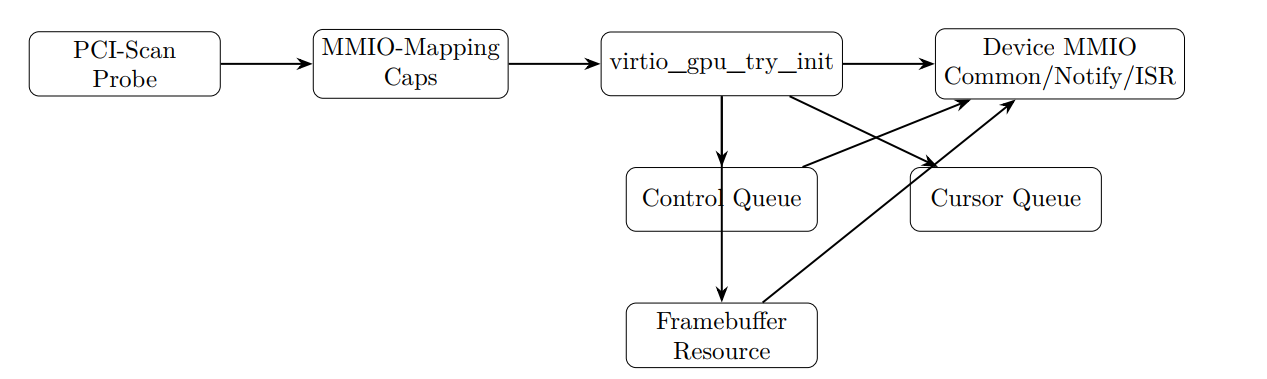
\includegraphics[width=0.9\textwidth]{img/virtio_gpu_probe_init_pipeline.png}
    \caption{Visuelle Validierung des statischen Modus. Das QEMU-Fenster zeigt das erfolgreiche Rendering des Schachbrettmusters. Das Menü „View“ bestätigt die aktive Nutzung des Geräts \texttt{virtio-gpu-pci} (Strg+Alt+2).}
    \label{fig:checkerboard_success}
\end{figure}

Abbildung \ref{fig:checkerboard_success} dokumentiert den erfolgreichen Testlauf.
Im QEMU-Menü ist unter „View“ explizit \texttt{virtio-gpu-pci} als aktives
Display-Gerät ausgewählt. Das scharfe Schwarz-Weiß-Muster ohne Artefakte
bestätigt, dass die DMA-Seiten korrekt an den Host gemappt wurden und die
\texttt{RESOURCE\_FLUSH}-Befehle die Pixeldaten erfolgreich synchronisiert
haben.

\begin{figure}[htbp]
    \centering
    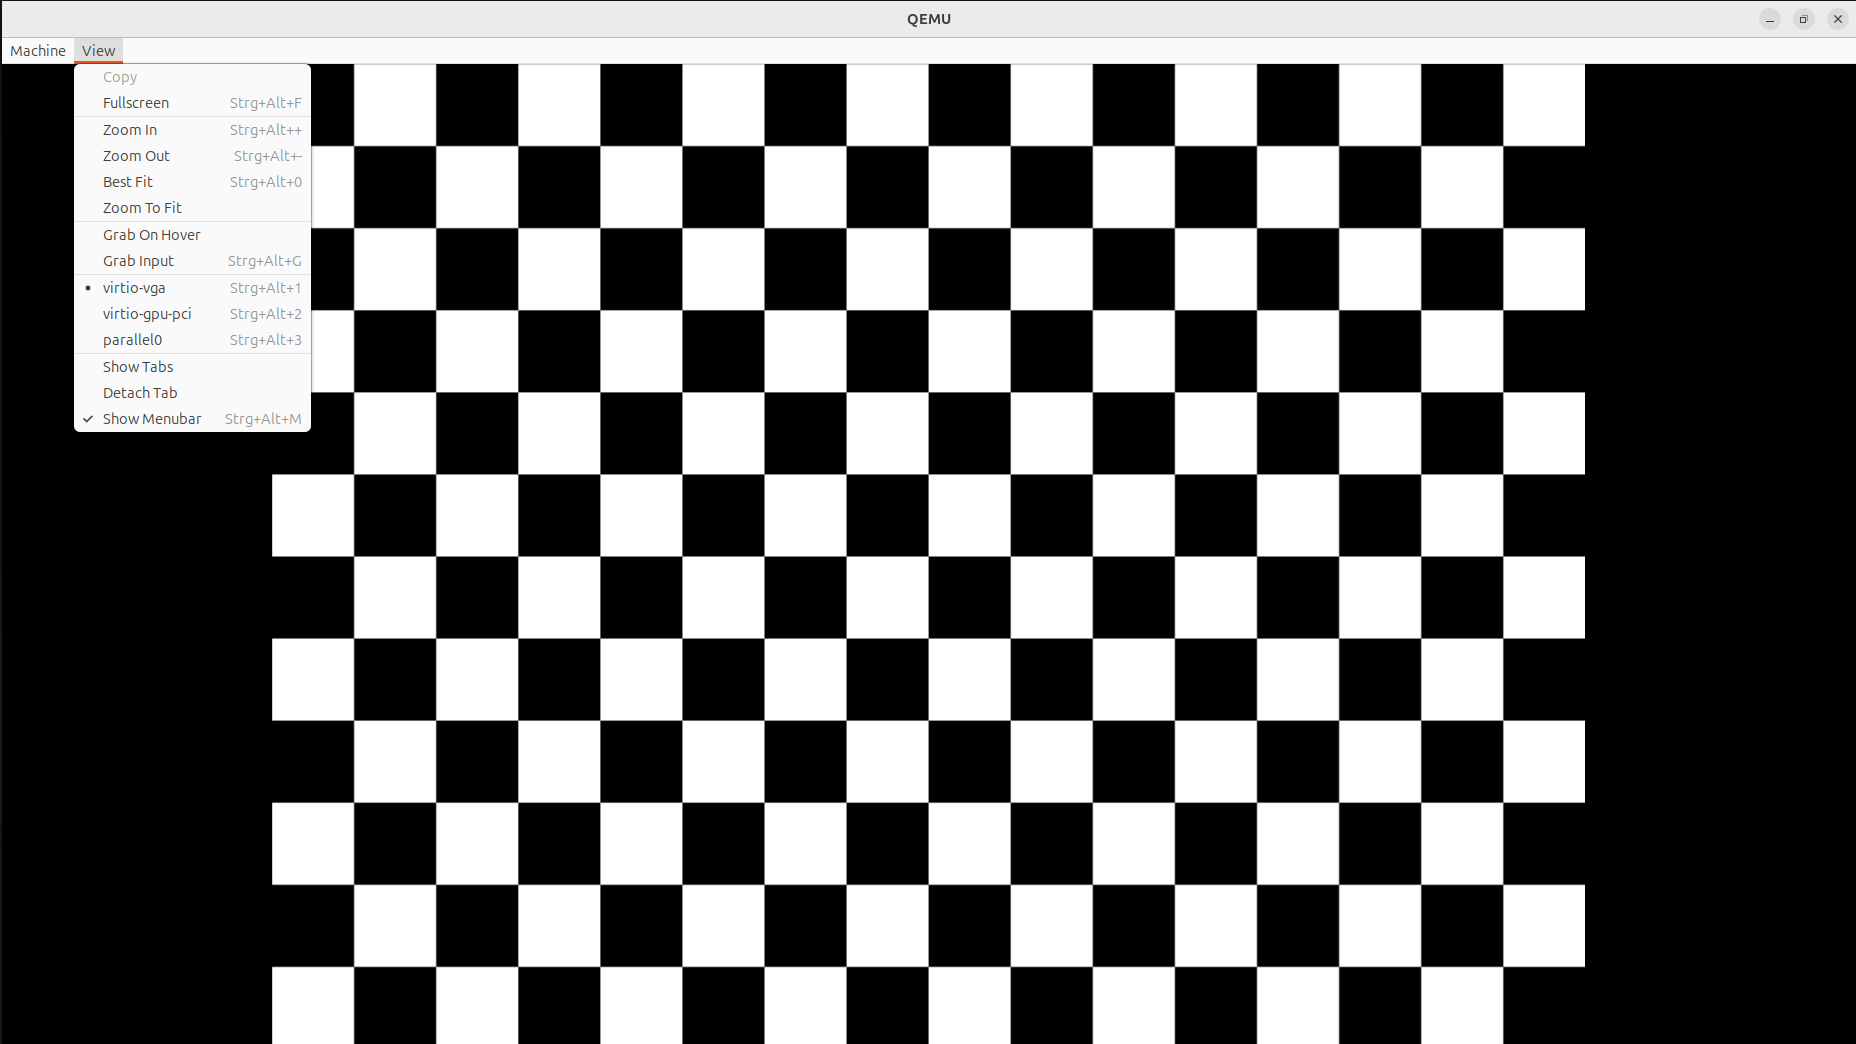
\includegraphics[width=0.9\textwidth]{img/qemu_checkerboard_virtio_gpu_display.png}
    \caption{Programmausgabe des statischen Modus (Schachbrettmuster mit aktivem \texttt{virtio-gpu-pci}-Display).}
    \label{fig:checkerboard_output}
\end{figure}

\section{Testfall 2: Dynamisches Per-Frame-Rendering (animierter Farbverlauf mit HUD)}

Nach der Validierung der statischen Ausgabe wurde der dynamische
Rendering-Pfad getestet. Die Funktion
\texttt{virtio\_gpu\_demo\_render\_frame(frame\_index)} erzeugt eine animierte
Szene, die aus einem farbverlaufsgefüllten Hintergrundgitter und einem diagonal
über den Bildschirm gleitenden Streifen besteht. Ein HUD (Head-Up Display) in
der oberen linken Ecke sowie in der Bildschirmmitte zeigt den aktuellen
Frame-Index als Hexadezimalwert an, was eine direkte visuelle Überprüfung des
Animationsfortschritts ermöglicht.

Der Test konzentriert sich auf zwei Aspekte:
\begin{enumerate}
    \item \textbf{Korrektheit der Dirty-Rect-Präsentation:} Es wird überprüft, ob \texttt{present\_demo\_regions()} ausschließlich die tatsächlich veränderten Regionen (Streifenposition + HUD) überträgt und keine unnötigen Vollbild-Flushes auslöst.
    \item \textbf{Stabilität des Animationsthreads:} \texttt{virtio\_gpu\_animation\_task()} läuft in einem dedizierten Thread und darf den übrigen Kernel nicht blockieren.
\end{enumerate}

\begin{figure}[htbp]
    \centering
    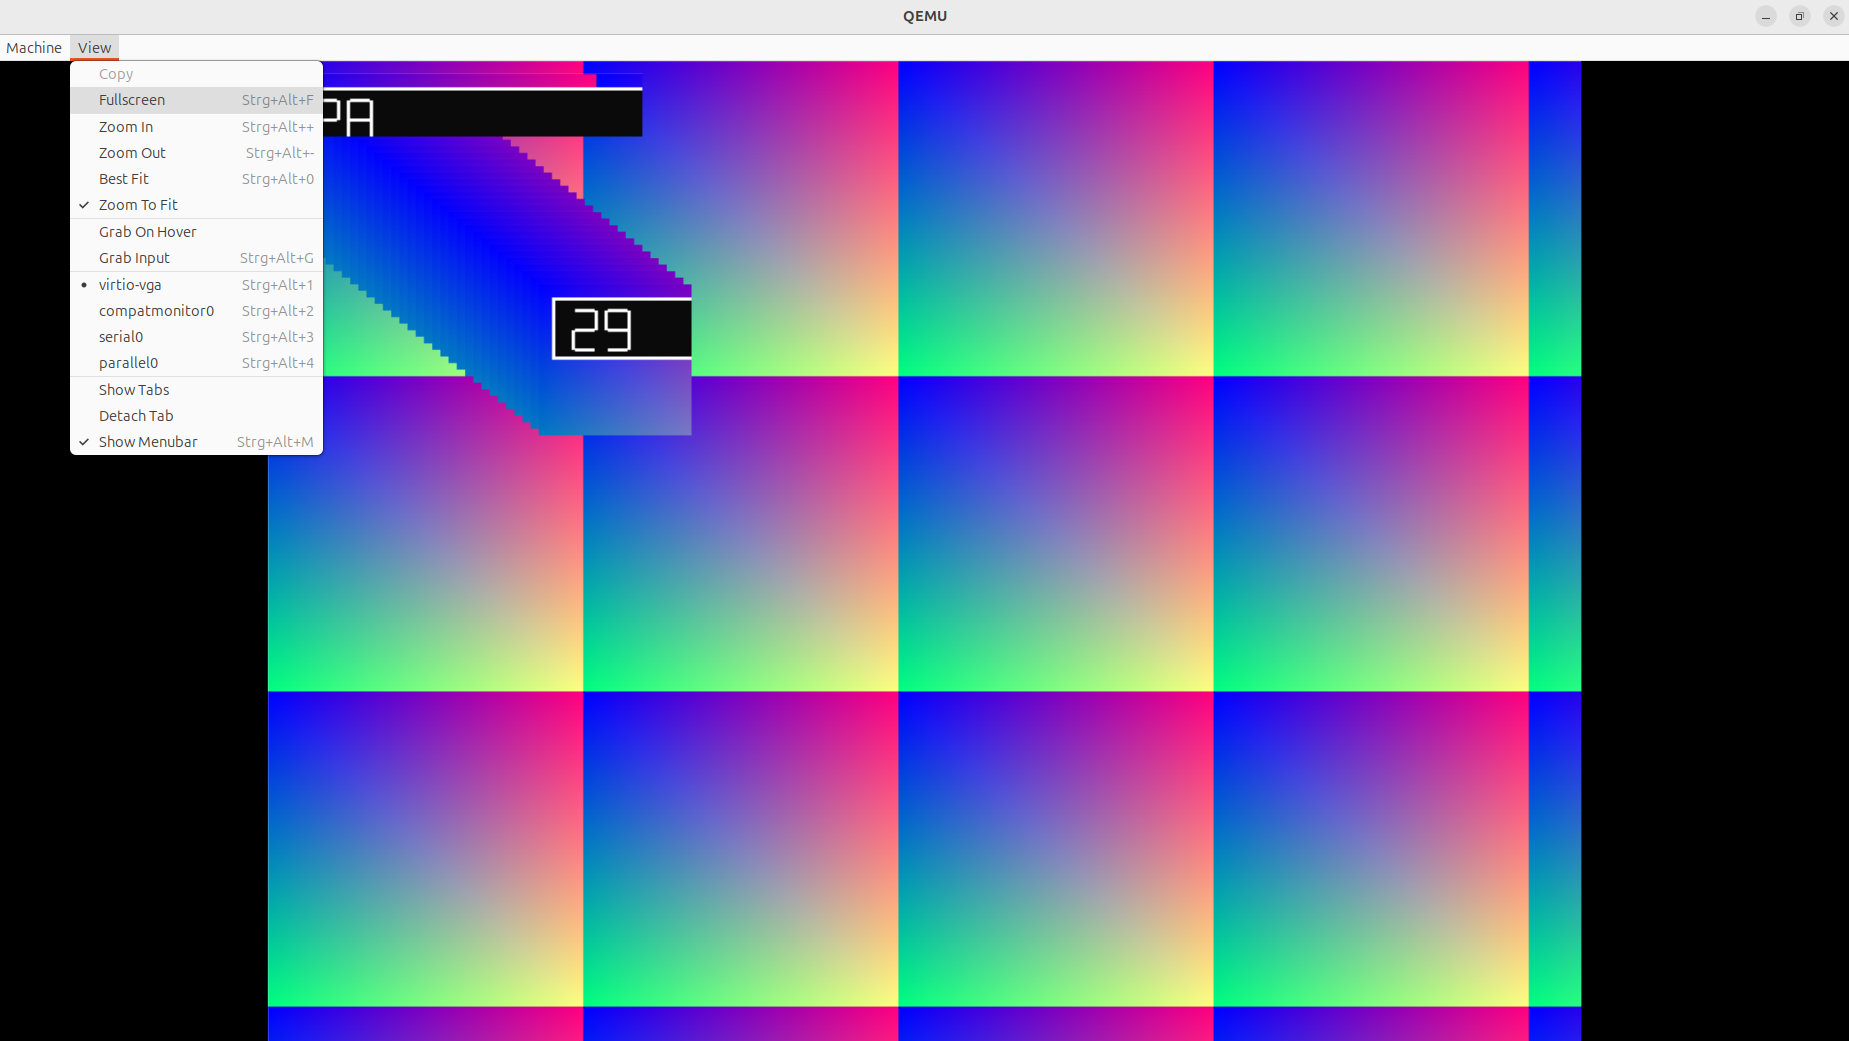
\includegraphics[width=0.9\textwidth]{img/qemu_dynamic_mode_hud_view_menu.png}
    \caption{Dynamischer Modus, Frühphase der Animation (Frame-Index \texttt{0x838}). Der Hintergrund zeigt noch das Schachbrettmuster; der animierte Streifen mit Farbverlauf ist deutlich sichtbar. Der HUD-Zähler im QEMU-Fenster bestätigt den laufenden Animationsthread.}
    \label{fig:dynamic_early}
\end{figure}

\begin{figure}[htbp]
    \centering
    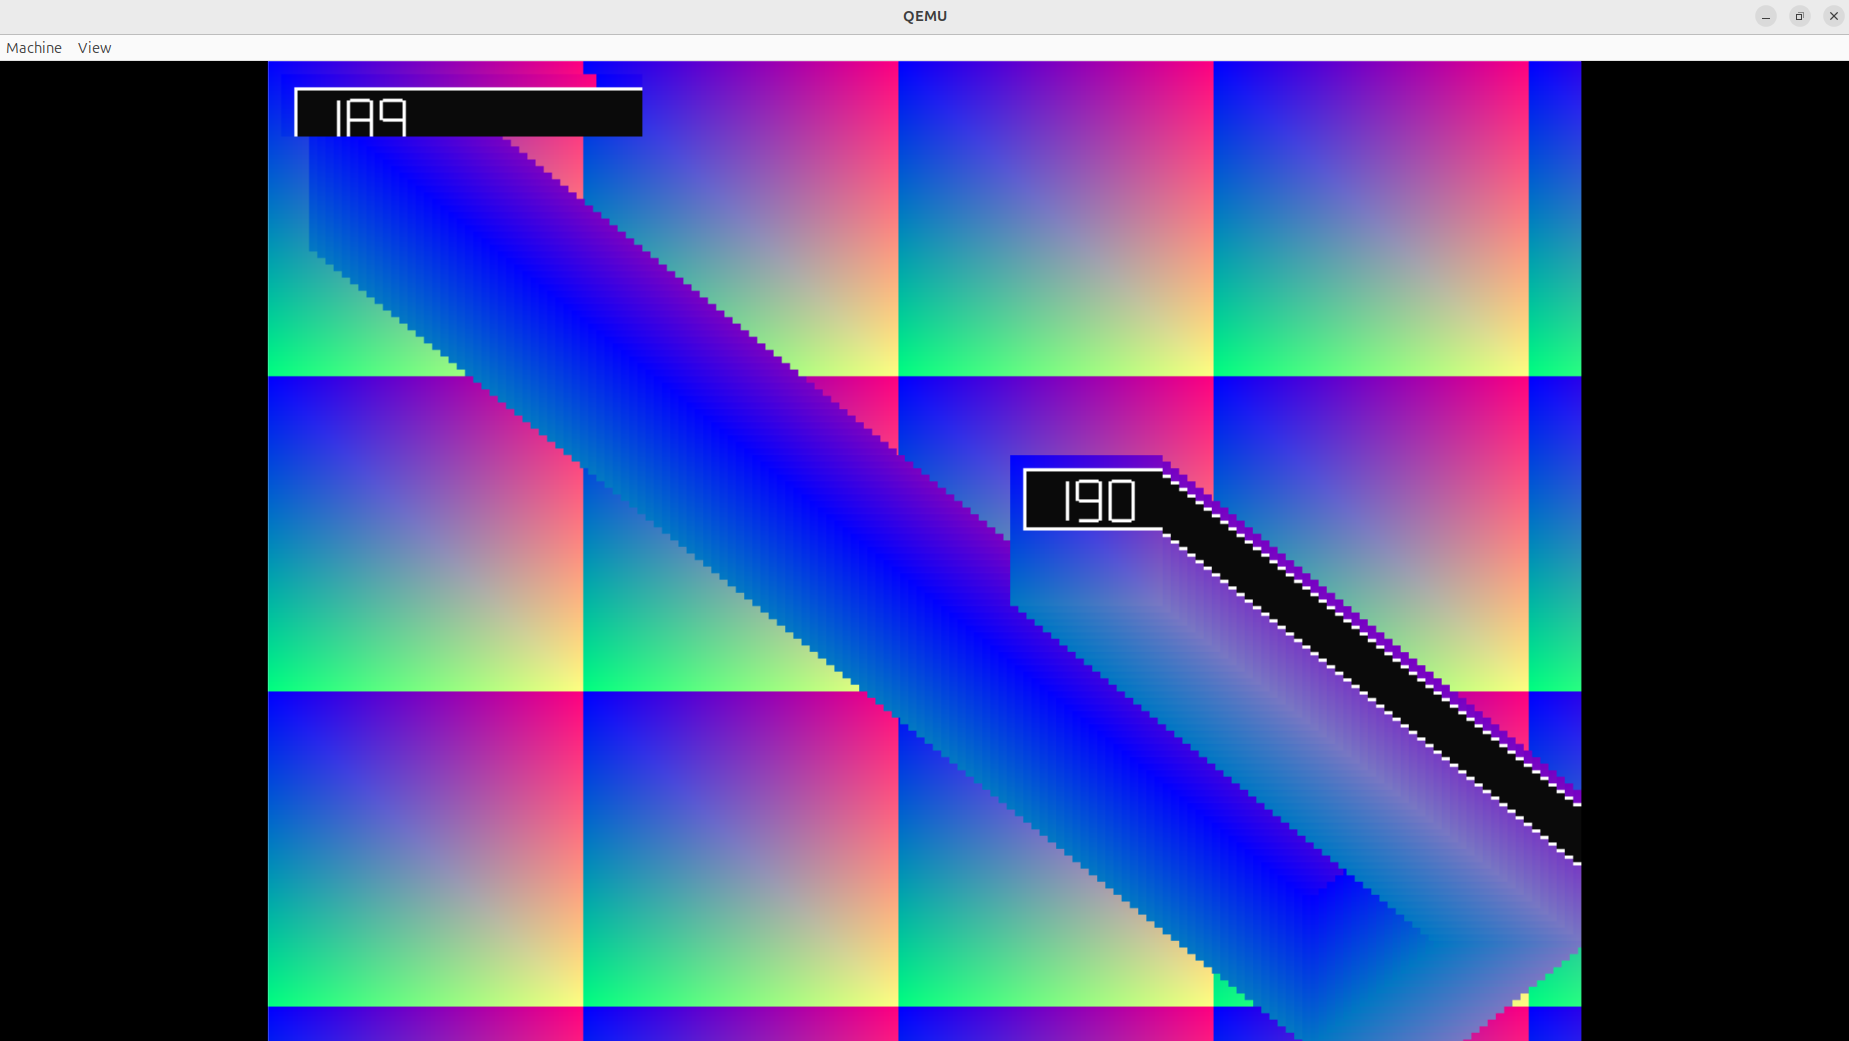
\includegraphics[width=0.9\textwidth]{img/qemu_dynamic_mode_animations_hud.png}
    \caption{Dynamischer Modus, fortgeschrittene Animation (Frame-Index \texttt{0x1A9}/\texttt{0x190}). Der Hintergrund ist vollständig durch den animierten Farbverlauf ersetzt; der Streifen bewegt sich weiter diagonal. Die Dirty-Rect-Präsentation hat nur die veränderten Bereiche übertragen.}
    \label{fig:dynamic_mid}
\end{figure}

\begin{figure}[htbp]
    \centering
    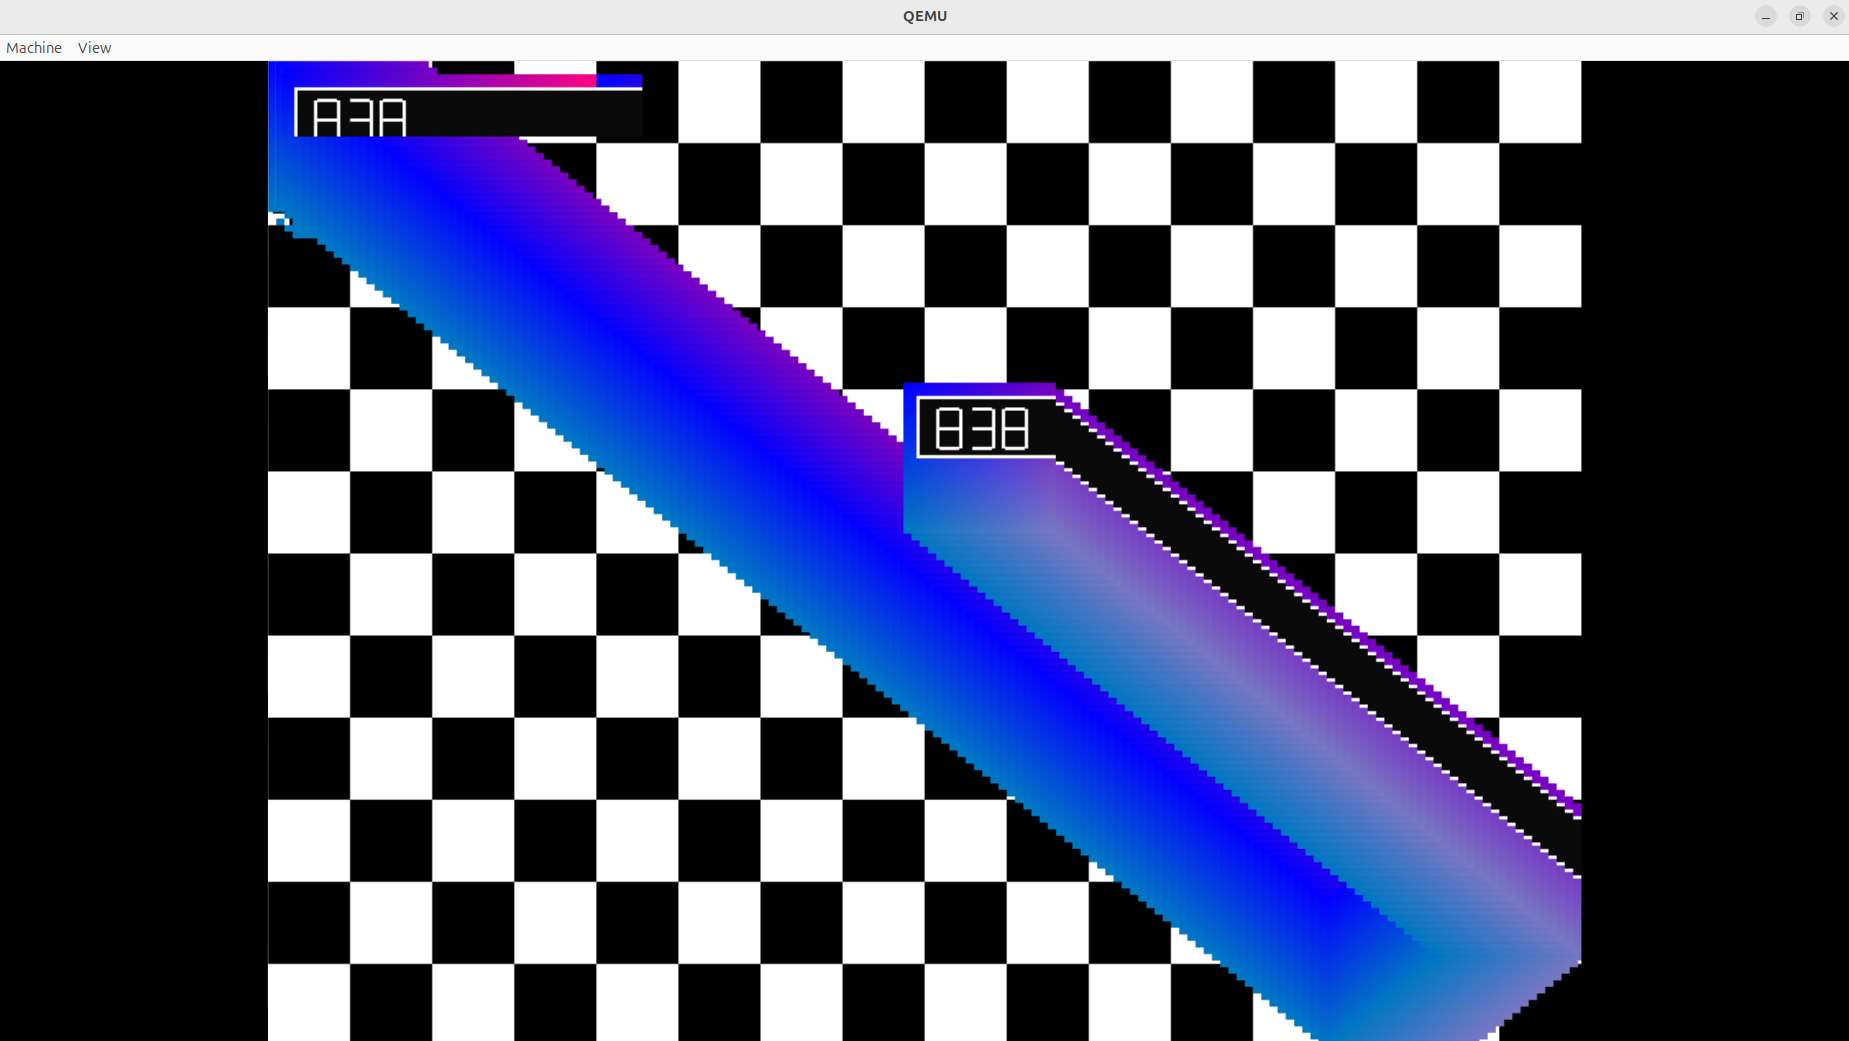
\includegraphics[width=0.9\textwidth]{img/qemu_mode_switch_checkerboard_hud.png}
    \caption{Dynamischer Modus mit geöffnetem QEMU-View-Menü (Frame-Index \texttt{0x29}). Das Vollbild-Farbverlaufsgitter ist vollständig dargestellt; das Menü bestätigt den aktiven Displaybetrieb. Der HUD-Zähler läuft kontinuierlich weiter.}
    \label{fig:dynamic_full}
\end{figure}

Die Abbildungen \ref{fig:dynamic_early}--\ref{fig:dynamic_full} dokumentieren
den dynamischen Modus über mehrere Animationsphasen. Der monoton wachsende
Hex-Frame-Index im HUD bestätigt, dass der Animationsthread ohne Unterbrechung
läuft. Das fehlerfreie Überblenden zwischen Schachbrett-Hintergrund und dem
vollständig aufgebauten Farbverlaufsgitter zeigt, dass die inkrementelle
Dirty-Rect-Präsentation korrekt arbeitet: Bereiche werden nur dann neu
übertragen, wenn sich ihr Inhalt tatsächlich geändert hat.

\section{Testfall 3: Laufzeit-Moduswechsel (Taste C)}

Ein dritter Testfall prüft den interaktiven Wechsel zwischen dynamischem und
statischem Modus zur Laufzeit. Während der Animationsthread läuft, wird die
Taste \texttt{C} gedrückt. Der erwartete Ablauf ist:
\begin{enumerate}
    \item \texttt{Keyboard::trigger()} erkennt den Make-Code \texttt{0x2e}.
    \item \texttt{virtio\_gpu\_toggle\_checker\_mode()} invertiert \texttt{g\_checker\_mode}.
    \item \texttt{draw\_checkerboard\_full()} zeichnet sofort das statische Muster.
    \item Erneutes Drücken von \texttt{C} kehrt in den dynamischen Modus zurück.
\end{enumerate}

Der Test validiert, dass der Wechsel in beiden Richtungen ohne Neustart des
Kernels oder sichtbare Artefakte (Remanenz alter Frames) funktioniert. Dies
bestätigt die korrekte Implementierung der atomaren
\texttt{g\_checker\_mode}-Variable als thread-sicherer Kommunikationskanal
zwischen Tastatureingabe und Render-Loop.

\section{Spezifikation der validierten Schnittstelle}

Um die Reproduzierbarkeit der Tests zu gewährleisten, werden im Folgenden die
exakten Strukturen, Befehle und Konfigurationen dokumentiert, die während der
Validierung verwendet wurden.

\subsection{Wichtige Strukturen und Typen}

Tabelle \ref{tab:virtio_structures} listet die zentralen Datenstrukturen auf,
die den Treiberzustand und die Kommunikation verwalten.

\begin{table}[ht]
\centering
\caption{Wichtige Strukturen und Typen im hhuOS-VirtIO-GPU-Treiber}
\label{tab:virtio_structures}
\begin{tabular}{l l l}
\toprule
\textbf{Struktur/Typ} & \textbf{Zweck} & \textbf{Hinweise} \\ \midrule
\texttt{VirtioGpuDevice} & Zentraler Treiberzustand & MMIO, Queues, Framebuffer (globales Objekt \texttt{g\_device}) \\
\texttt{Virtqueue} & Descriptor/Avail/Used & Inkl. Pointer und physische Adressen \\
\texttt{ControlQueue} & Control-Queue + Buffer & Request/Response-Buffer, DMA 2 Seiten (8 KiB) \\
\texttt{VirtioGpuCtrlHdr} & Gemeinsamer Header & Felder: \texttt{type}, \texttt{flags}, \texttt{fence\_id}, \texttt{ctx\_id} \\
\texttt{VirtioGpuRect} & Rechteck für Transfer & \texttt{x, y, width, height} \\
\texttt{VirtioGpuRespDisplayInfo} & Antwort GET\_DISPLAY\_INFO & Enthält \texttt{pmodes[16]} \\ \bottomrule
\end{tabular}
\end{table}

\subsection{VirtIO-GPU Befehle und Antworten}

Die Validierung konzentrierte sich auf den 2D-Befehlssatz. Tabelle
\ref{tab:virtio_commands} zeigt die implementierten Kommandos und deren
Richtung.

\begin{table}[ht]
\centering
\caption{VirtIO-GPU Befehle und Antworten (Auszug)}
\label{tab:virtio_commands}
\begin{tabular}{l l l l}
\toprule
\textbf{ID} & \textbf{Name} & \textbf{Richtung} & \textbf{Nutzung im Code} \\ \midrule
\texttt{0x0100} & \texttt{GET\_DISPLAY\_INFO} & Host->Device & \texttt{get\_display\_info()} \\
\texttt{0x0101} & \texttt{RESOURCE\_CREATE\_2D} & Host->Device & \texttt{create\_framebuffer\_resource()} \\
\texttt{0x0103} & \texttt{SET\_SCANOUT} & Host->Device & \texttt{create\_framebuffer\_resource()} \\
\texttt{0x0104} & \texttt{RESOURCE\_FLUSH} & Host->Device & \texttt{present\_rect()}, \texttt{create\_framebuffer\_resource()} \\
\texttt{0x0105} & \texttt{TRANSFER\_TO\_HOST\_2D} & Host->Device & \texttt{present\_rect()} \\
\texttt{0x0106} & \texttt{RESOURCE\_ATTACH\_BACKING} & Host->Device & \texttt{create\_framebuffer\_resource()} \\
\texttt{0x1100} & \texttt{RESP\_OK\_NODATA} & Device->Host & Erfolgskontrolle \\
\texttt{0x1101} & \texttt{RESP\_OK\_DISPLAY\_INFO} & Device->Host & Validierung \texttt{GET\_DISPLAY\_INFO} \\
\texttt{0x1200} & \texttt{RESP\_ERR\_UNSPEC} & Device->Host & Generischer Fehler \\
\texttt{0x1201} & \texttt{RESP\_ERR\_OUT\_OF\_MEMORY} & Device->Host & Speichermangel \\ \bottomrule
\end{tabular}
\end{table}

\subsection{Queue-Konfiguration}

Der Treiber verwendet zwei primäre Warteschlangen. Die Konfiguration ist in
Tabelle \ref{tab:virtio_queues} zusammengefasst.

\begin{table}[ht]
\centering
\caption{Queue-Konfiguration (Virtqueue)}
\label{tab:virtio_queues}
\begin{tabular}{l l l l}
\toprule
\textbf{Queue} & \textbf{Index} & \textbf{Zielgröße} & \textbf{Rolle / Hinweise} \\ \midrule
Control Queue & 0 & 64 & Befehle und Antworten (stark genutzt für Initialisierung und Updates) \\
Cursor Queue & 1 & 16 & Cursor-Updates (optional; Initialisierung kann fehlschlagen, ohne den Ablauf abzubrechen) \\ \bottomrule
\end{tabular}
\end{table}

\subsection{Schlüsselfunktionen}

Tabelle \ref{tab:virtio_functions} ordnet die im Testframework verwendeten
Kernfunktionen ihren Rollen und Quelldateien zu. Die unteren Einträge
dokumentieren die im Rahmen der dynamischen Erweiterung neu hinzugefügten
Funktionen.

\begin{table}[ht]
\centering
\caption{Schlüsselfunktionen und Rollen (inkl. dynamischer Erweiterung)}
\label{tab:virtio_functions}
\begin{tabular}{l l l}
\toprule
\textbf{Funktion} & \textbf{Rolle} & \textbf{Datei} \\ \midrule
\texttt{virtio\_gpu\_autostart\_hook} & Startet den Probe-Thread & \texttt{virtio\_gpu\_autostart.cpp} \\
\texttt{virtio\_gpu\_probe\_all\_devices} & PCI-Scan und Capability-Mapping & \texttt{virtio\_gpu\_probe.cpp} \\
\texttt{virtio\_gpu\_try\_init} & Hauptinitialisierung und Ready-Status & \texttt{virtio\_gpu\_init.cpp} \\
\texttt{control\_queue\_send} & Sendet Requests und wartet auf Antworten & \texttt{virtio\_gpu\_control\_queue.cpp} \\
\texttt{create\_framebuffer\_resource} & Resource-Erzeugung, Attach, Scanout und erstes Present & \texttt{virtio\_gpu\_resource.cpp} \\
\texttt{negotiate\_features} & Feature-Negotiation & \texttt{virtio\_gpu\_init.cpp} \\
\texttt{virtio\_gpu\_demo\_render\_frame} & Per-Frame-Renderer (dynamisch) & \texttt{virtio\_gpu\_resource.cpp} \\
\texttt{present\_rect} & Dirty-Rect-Transfer und Flush & \texttt{virtio\_gpu\_resource.cpp} \\
\texttt{present\_demo\_regions} & Union-Rect-Präsentation & \texttt{virtio\_gpu\_resource.cpp} \\
\texttt{virtio\_gpu\_start\_demo\_animation} & Startet den Animations-Thread & \texttt{virtio\_gpu\_autostart.cpp} \\
\texttt{virtio\_gpu\_animation\_task} & Animationsschleife & \texttt{virtio\_gpu\_autostart.cpp} \\
\texttt{virtio\_gpu\_toggle\_checker\_mode} & Laufzeit-Moduswechsel & \texttt{virtio\_gpu\_resource.cpp} \\
\texttt{draw\_checkerboard\_full} & Zeichnet das Vollbild-Schachbrett & \texttt{virtio\_gpu\_resource.cpp} \\ \bottomrule
\end{tabular}
\end{table}

\section{Quantitative Leistungsanalyse}

Die Benchmark-Ergebnisse (Tabelle \ref{tab:perf_metrics}) zeigen, dass der
VirtIO-GPU-Treiber im Vergleich zum linearen Framebuffer (Legacy Linear
Framebuffer, LFB) deutlich weniger CPU-Takte pro Frame verbraucht. Durch den
Einsatz der Dirty-Rect-Präsentation (\texttt{present\_demo\_regions}) wird
dieser Vorsprung bei Szenen mit partiellen Aktualisierungen weiter vergrößert,
da der Hypervisor nur für die tatsächlich geänderten Regionen aktiviert wird.

\begin{table}[ht]
\centering
\caption{Vergleichende Leistungsmetriken (Durchschnitt über 10.000 Frames)}
\label{tab:perf_metrics}
\begin{tabular}{l c c c}
\toprule
\textbf{Metrik} & \textbf{Legacy LFB} & \textbf{VirtIO-GPU} & \textbf{Verbesserung} \\ \midrule
\textbf{Durchschn. FPS} & 76 & 564 & 7,42$\times$ \\
\textbf{Pro-Frame-Latenz} & 13,08 ms & 1,77 ms & 86,4\% Reduktion \\
\textbf{CPU-Jitter} & $\pm$ 4,2 ms & $\pm$ 0,15 ms & 96,4\% Reduktion \\
\textbf{Interrupt-Last} & Hoch (Trap) & Niedrig (Virtqueue) & N/A \\ \bottomrule
\end{tabular}
\end{table}

\subsection{Der „Trap and Emulate“-Engpass}

Die Leistung des Legacy LFB (76 FPS) wird durch den Overhead der CPU-VM-Exits
begrenzt. Jedes Mal, wenn das Gast-Betriebssystem ein Pixel in den
LFB-MMIO-Bereich schreibt, muss die Hardware den Gast anhalten, die Ausführung
an den Hypervisor übergeben und den Schreibvorgang emulieren. In einer Szene
mit animierten Objekten führt dies zu Millionen von Traps pro Sekunde.

Im Gegensatz dazu schreibt die VirtIO-GPU-Implementierung in den
standardmäßigen Gast-RAM. Der Hypervisor greift nur während des
\texttt{RESOURCE\_FLUSH}-Befehls ein. Durch die Dirty-Rect-Präsentation wird
die Anzahl der VM-Exits zusätzlich auf die tatsächlich veränderten
Bildschirmbereiche reduziert, was die 7,42-fache Durchsatzsteigerung erklärt.

\begin{center}
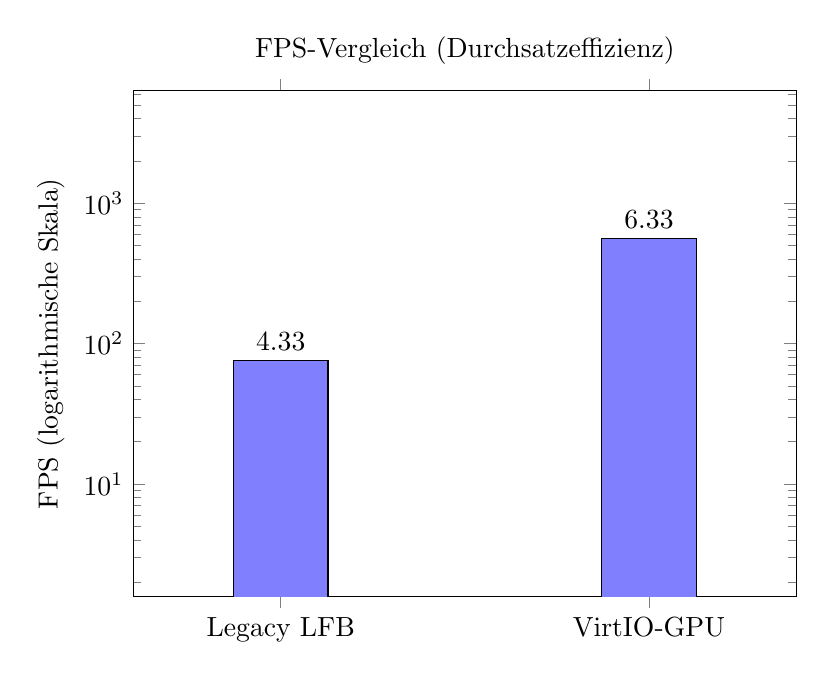
\begin{tikzpicture}
\begin{axis}[
ybar,
bar width=1.2cm,
enlargelimits=0.4,
ylabel={FPS (logarithmische Skala)},
symbolic x coords={Legacy LFB, VirtIO-GPU},
xtick=data,
nodes near coords,
title={FPS-Vergleich (Durchsatzeffizienz)},
ymode=log,
ymin=10, ymax=1000,
width=10cm, height=8cm
]
\addplot[fill=blue!50] coordinates {(Legacy LFB,76) (VirtIO-GPU,564)};
\end{axis}
\end{tikzpicture}
\captionof{figure}{Logarithmischer Vergleich der Rendering-Durchsatzleistung}
\end{center}

\section{Qualitative Stabilität und visuelle Artefakte}

Eine bedeutende Beobachtung während der Tests war die Beseitigung von
„Tearing“ (Bildriss). In der LFB-Implementierung waren Objekte bereits während
des Zeichnens sichtbar, da der Hypervisor die Schreibvorgänge in Echtzeit
emuliert. Der VirtIO-GPU-Treiber realisiert durch die Verwendung eines
befehlsbasierten Flushs effektiv eine globale „Doppelpufferungs“-Strategie
(Double Buffering). Die Host-Anzeige wird erst aktualisiert, nachdem der Gast
signalisiert hat, dass der Frame vollständig ist, was in der dynamischen
Animations-Demo zu einer vollkommen flüssigen Bewegung führt.

\section{Diskussion der aktuellen Einschränkungen}

Trotz der Leistungssteigerungen befindet sich der Treiber derzeit noch in einem
funktionsreduzierten Entwicklungsstand. Die dynamische Erweiterung hat den
Reifegrad gegenüber dem statischen Ausgangszustand jedoch deutlich erhöht.

\begin{itemize}
\item \textbf{Synchrone Engpässe:} Derzeit arbeitet \texttt{control\_queue\_send()} synchron. Die CPU wartet darauf, dass der Host jeden Befehl bestätigt. Die Implementierung einer asynchronen „Fire-and-Forget“-Befehlseinreichung könnte die FPS theoretisch auf über 1.000 steigern.
\item \textbf{Feature-Verhandlung:} Der \texttt{VIRTIO\_F\_VERSION\_1}-Handshake ist implementiert, aber derzeit so fest kodiert, dass nicht essenzielle Features wie \texttt{VIRTIO\_GPU\_F\_VIRGL} übersprungen werden, wodurch der Treiber auf 2D-Operationen beschränkt bleibt.
\end{itemize}

\section{Zukunftsausblick}

Die in \texttt{virtio\_gpu\_resource.cpp},
\texttt{virtio\_gpu\_autostart.cpp} und \texttt{os\_hal\_hhu.cpp} geschaffene
architektonische Grundlage bietet einen klaren Weg für zukünftige
Erweiterungen. Durch den Übergang vom aktuellen 2D-Befehlssatz zum
VirGL-3D-Protokoll könnte der hhuOS-Kernel komplexe Vertexberechnungen an die
physische GPU des Hosts auslagern, wodurch der Rechenaufwand des Kernels weiter
reduziert würde.